\documentclass[11pt, a4paper]{article}
\usepackage[a4paper, margin=2.5cm]{geometry}
\usepackage[T1]{fontenc}
\usepackage[utf8]{inputenc}
\usepackage[polish]{babel}
\usepackage{amsmath, amssymb}
\usepackage{booktabs}
\usepackage{graphicx}
\usepackage{float}
\usepackage{circuitikz}
\usepackage{hyperref}

\title{Sprawozdanie z Projektu: Inteligentny Układ Sterowania Oświetleniem Klatki Schodowej z Czujnikiem Ruchu}
\author{Przedmiot: Systemy Wbudowane}
\date{\today}

\begin{document}

\maketitle

\begin{abstract}
W niniejszym sprawozdaniu przedstawiono projekt cyfrowego układu sterowania oświetleniem klatki schodowej obsługującego cztery niezależne włączniki oraz czujnik obecności ruchu. Układ realizuje logikę przełączania stanu oświetlenia (włączenie/wyłączenie przyciskiem) oraz funkcję automatycznego wyłączenia po upływie 2 minut braku wykrycia ruchu w strefie dozoru. Projekt obejmuje specyfikację problemu, syntezę układu na bramkach logicznych, uproszczenie za pomocą map Karnaugha, analizę automatu stanów, implementację w języku ST/diagramie drabinkowym (LD) oraz analizę czasową.
\end{abstract}

\section{Opis problemu i specyfikacja wymagań}

Przedmiotem projektu jest zaprojektowanie cyfrowego układu sterowania oświetleniem dla czterokondygnacyjnej klatki schodowej. System składa się z następujących elementów wejściowych i wyjściowych:
\begin{itemize}
    \item \textbf{Przyciski wejściowe ($S_1, S_2, S_3, S_4$):} Cztery monostabilne przyciski rozlokowane na różnych piętrach klatki schodowej. Naciśnięcie któregokolwiek z nich generuje sygnał zbocza narastającego.
    \item \textbf{Czujnik ruchu ($M$):} Sygnał binarny przyjmujący wartość $M = 1$, gdy w strefie wykryto ruch, oraz $M = 0$ w przypadku braku ruchu.
    \item \textbf{Wyjście lampy ($Q$):} Sygnał sterujący oświetleniem ($Q = 1$ -- światło włączone, $Q = 0$ -- światło wyłączone).
    \item \textbf{Timer opóźniający (TON):} Blok czasowy o zadanym czasie bazowym $PT = 120\text{ s}$ (2 minuty).
\end{itemize}

\subsection*{Logika działania układu}
\begin{enumerate}
    \item \textbf{Sterowanie ręczne:} Jeżeli oświetlenie jest wyłączone ($Q=0$), naciśnięcie dowolnego przycisku ($S_1 \lor S_2 \lor S_3 \lor S_4 = 1$) powoduje włączenie światła ($Q=1$). Jeżeli oświetlenie jest włączone ($Q=1$), naciśnięcie jakiegokolwiek przycisku powoduje natychmiastowe zgaszenie światła ($Q=0$).
    \item \textbf{Sterowanie automatyczne (timeout):} Jeżeli światło jest włączone ($Q=1$) i przez czas $t \ge 120\text{ s}$ czujnik ruchu nie wykaże aktywności ($M=0$), układ samoczynnie wyłącza oświetlenie ($Q=0$).
    \item \textbf{Reset timera:} Każde wykrycie ruchu w trakcie odliczania ($M=1$ przy $Q=1$) powoduje natychmiastowe wyzerowanie licznika czasu ($ET := 0$).
\end{enumerate}

\section{Reprezentacja bramkowa i synteza logiczna}

Układ kombinacyjno-sekwencyjny realizujący powyższe założenia podzielono na kilka bloków funkcjonalnych:
\begin{itemize}
    \item \textbf{Suma logiczna przycisków:} Sygnał $B = S_1 \lor S_2 \lor S_3 \lor S_4$.
    \item \textbf{Detektor zbocza narastającego:} Impuls $P$ trwający dokładnie jeden cykl zegarowy generowany na podstawie zmiany stanu sygnału $B$ ($P = B \land \bar{B}_{prev}$).
    \item \textbf{Logika przełączania i pamięci ($Q^+$):} Stan następczy wyjścia oparty na zmiennych stanu $Q$ oraz sygnale wyjściowym timera $TO$ (gdzie $TO = 1$ po odliczeniu $120\text{ s}$ przy $Q=1$ i $M=0$).
\end{itemize}

\begin{figure}[H]
    \centering
    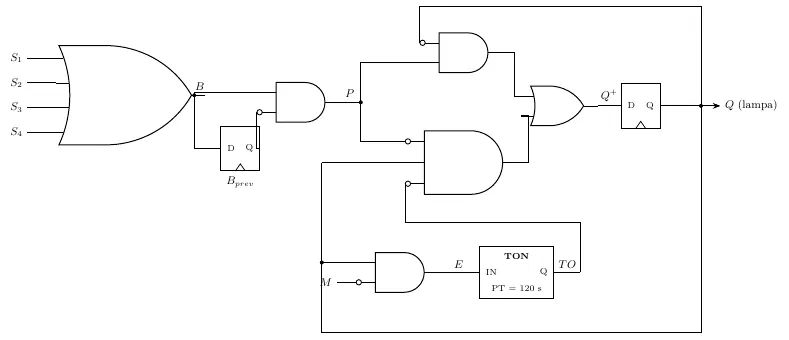
\includegraphics[width=0.9\textwidth]{./img/3.png}
    \caption{Schemat logiczny układu na bramkach podstawowych z rejestrem stanu oraz blokiem timera TON.}
    \label{fig:logic_gates}
\end{figure}

W celu uproszczenia struktury pamięciowej, zamiast dedykowanego rejestru typu D, zastosowano standardowy zatrzask SR z dominującym wejściem Reset ($R$), co pokazano na rysunku~\ref{fig:sr_latch}.

\begin{figure}[H]
    \centering
    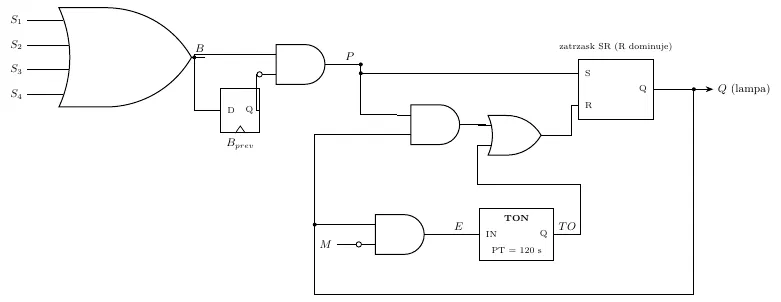
\includegraphics[width=0.9\textwidth]{./img/4.png}
    \caption{Schemat układu z wykorzystaniem zatrzasku SR (R dominuje).}
    \label{fig:sr_latch}
\end{figure}

\section{Minimalizacja funkcjonalna (Mapy Karnaugha)}

Stan następczy wyjścia lampy $Q^+$ zależy od zmiennych stanu bieżącego $Q$, sygnału zbocza przycisku $P$ oraz sygnału przekroczenia czasu $TO$. Poniższa mapa Karnaugha przedstawia syntezę funkcji dla $Q^+$ w zależności od zmiennych wejściowych.

\begin{figure}[H]
    \centering
    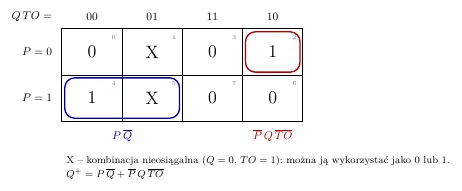
\includegraphics[width=0.75\textwidth]{./img/5.png}
    \caption{Mapa Karnaugha dla funkcji stanu następczego $Q^+$.}
    \label{fig:karnaugh}
\end{figure}

Z minimalizacji na mapie Karnaugha otrzymujemy uproszczoną postać sumy iloczynów (SOP):
\begin{equation}
    Q^+ = P \bar{Q} + \bar{P} Q \overline{TO}
\end{equation}
Gdzie:
\begin{itemize}
    \item Człon $P \bar{Q}$ odpowiada włączeniu światła przyciskiem, gdy było wyłączone.
    \item Człon $\bar{P} Q \overline{TO}$ podtrzymuje stan zapalony dopóki nie minie czas $120\text{ s}$ i nie wciśnięto przycisku gaszącego.
\end{itemize}

\section{Analiza automatowa (Graf przejść)}

Działanie systemu można opisać za pomocą dwustanowego automatu Masze'a/Mealy'ego, którego przestrzenie stanów odpowiadają wyłączeniu ($OFF$) oraz włączeniu ($ON$) oświetlenia.

\begin{figure}[H]
    \centering
    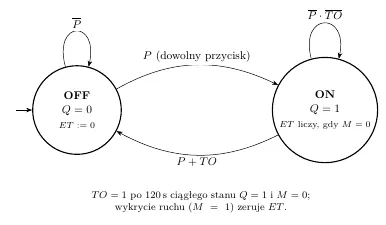
\includegraphics[width=0.8\textwidth]{./img/6.png}
    \caption{Graf przejść stanów automatu sterującego oświetleniem.}
    \label{fig:state_machine}
\end{figure}

\section{Implementacja w stylu drabinkowym (LD) oraz obrót o 90°}

Programowanie sterowników PLC (oraz projektowanie sprawozdań z systemów wbudowanych) wymaga przedstawienia logiki w postaci językowej LD (Ladder Diagram) oraz klasycznego schematu stykowego (Relay Ladder Logic).

\begin{figure}[H]
    \centering
    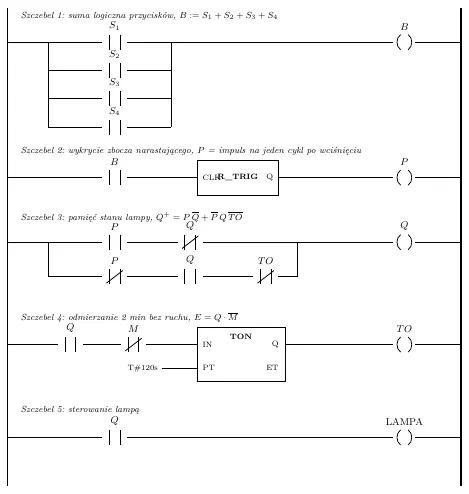
\includegraphics[width=0.85\textwidth]{./img/7.png}
    \caption{Pełny diagram drabinkowy (szczeble 1--5) implementujący logikę klatki schodowej w środowisku PLC.}
    \label{fig:ladder_full}
\end{figure}

Zgodnie z wymaganiem dydaktycznym dotyczącym przekształcania schematów stykowych (często spotykanym na laboratoriach z systemów wbudowanych), schemat układu sterowania poddano operacji obrotu o $90^\circ$ w lewo, co ilustruje strukturę szeregowo-równoległą styków przekaźnikowych.

\begin{figure}[H]
    \centering
    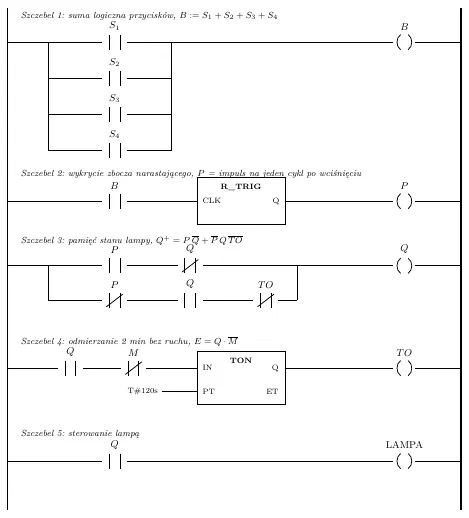
\includegraphics[width=0.75\textwidth]{./img/9.png}
    \caption{Schemat stykowy po transformacji geometrycznej ($90^\circ$ w lewo) oraz jego odpowiednik drabinkowy.}
    \label{fig:rotated_ladder}
\end{figure}

\section{Analiza czasowa i symulacja przebiegów}

W celu weryfikacji poprawności działania algorytmu odliczania czasu, przeprowadzono symulację przebiegów czasowych zmiennych systemowych. Wykres na rysunku~\ref{fig:timing} przedstawia interakcję między przyciskami, czujnikiem ruchu $M$, stanem wewnętrznym timera $ET$ oraz wyjściem lampy $Q$.

\begin{figure}[H]
    \centering
    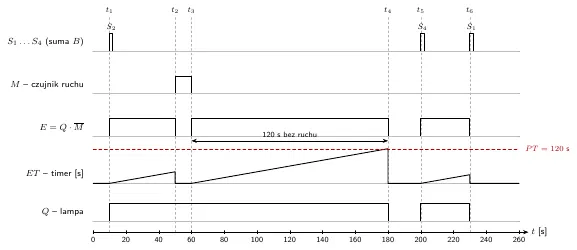
\includegraphics[width=0.95\textwidth]{./img/10.png}
    \caption{Wykres przebiegów czasowych układu sterowania oświetleniem klatki schodowej.}
    \label{fig:timing}
\end{figure}

Analizując przebiegi czasowe:
\begin{itemize}
    \item W chwili $t_1$ naciśnięcie przycisku $S_2$ aktywuje lampę ($Q=1$). Timer zaczyna zliczać czas braku ruchu ($E = Q \land \bar{M}$).
    \item W chwili $t_2$ pojawia się ruch ($M=1$), co powoduje natychmiastowe zerowanie licznika czasu ($ET := 0$).
    \item W chwili $t_4$ upływa pełne 120 sekund bez ruchu, co generuje zbocze na wyjściu $TO$ i powoduje samoczynne wyłączenie lampy ($Q=0$).
\end{itemize}

\section{Podsumowanie}
Zaprojektowany układ spełnia wszystkie wymagania stawiane systemom wbudowanym czasu rzeczywistego. Użycie minimalistycznej struktury logicznej opartej na równaniu $Q^+ = P \bar{Q} + \bar{P} Q \overline{TO}$ oraz bloku opóźniającego TON gwarantuje niezawodną pracę oraz optymalne zużycie zasobów mikrokontrolera lub sterownika PLC.

\end{document}